\documentclass{math}

\title{Funktionalanalysys}
\author{Patrick Jenny}
\date{\today}

\begin{document}
	\maketitle
	
	\tableofcontents
	\newpage
	
	
	%------1-HILBERTRÄUME------%
	\section{Hilberträume}
    \begin{Def}
		Ein metrischer Raum besteht aus eine Menge $X$ und einer Abb. $d: X,X\rightarrow \mathbb{R}$
		die jedem geordneten Paar von Elementen aus $X$ eine reele Zahl Zuordnet.

		Diese Abb soll ($\forall x,y,z \in X$) folgende Eigenschaften bessitzen:

		\begin{itemize}
			\item $d(x,y) \geq 0$ (Nichtnegativität)
			\item $d(x,y) = 0 \Leftrightarrow x = y$ (Eindeutigkeit)
			\item $d(x,y) = d(y,x)$ (Symetrie)
			\item $d(x,y) + d(y,z) \geq d(x,z)$ (Dreiecksungleichung)
		\end{itemize}
	\end{Def}
	
	\begin{Def}
		Ein normierter Raum ist ein Vektorraum $V$ über den Köprer $\mathbb{C} (\mathbb{R})$
		auf dem eine Abb. $\Vert\cdot\Vert: V \rightarrow \mathbb{R}$ erklärt ist, die jedem
		Element $x \in V$ eine reele Zahl $\Vert x \Vert$ zuordnet und folgende Eigenschaften
		besitzt
		\begin{itemize}
			\item $\Vert x \Vert \geq 0$ (Nichtnegativität)
			\item $\Vert x \Vert = 0 \Leftrightarrow x = 0$ (Eindeutigkeit)
			\item $\Vert \alpha \cdot x \Vert = \vert \alpha \vert \cdot \Vert x \Vert$ (Skalierung)
			\item $\Vert x + y\Vert \leq \Vert x \Vert + \Vert y \Vert$ (Dreiecksungleichung)
		\end{itemize}
	\end{Def}

	\begin{Bem}
		Jeder normierte Raum ist ein metrischer Raum mit Metrik $d(x,y) = \Vert x-y \Vert$
		durch die Norm induzierte Metrik. 
	\end{Bem}

	\begin{Def}
		Ein normierter Raum, in dem jede Cauchy-Folge konvergiert (bzgl. Metrik $d(x,y) = \Vert x-y \Vert$)
		ist ein vollständig normierter Raum bzw. Banachraum.
	\end{Def}

	% \begin{Bsp}
	% 	\begin{itemize}
	% 		\item $\mathbb{R}^n: \Vert \vec x \Vert = \sqrt{\sum_{i=1}^n x_i^2}$
	% 		\item $\mathbb{C}^n: \Vert \vec z \Vert = \sqrt{\sum_{i=1}^n z_i^2}$
	% 		\item Hilbert'scher Folgenraum $\ell^2$
	% 	\end{itemize}
	% \end{Bsp}

	\textbf{Beispiele}
	\begin{itemize}
		\item $\mathbb{R}^n: \Vert \vec x \Vert = \sqrt{\sum_{i=1}^n x_i^2}$
		\item $\mathbb{C}^n: \Vert \vec z \Vert = \sqrt{\sum_{i=1}^n z_i^2}$
		\item Hilbert'scher Folgenraum $\ell^2$
	\end{itemize}

	\begin{Def}
		Sei $V$ ein Vektorraum über $\mathbb{C} (\mathbb{R})$.
		Ein Skalarprodukt auf $V$ ist eine Abb. die jedem geordneten Paar von
		Elementen aus $V$ eindeutig ein, mit $\langle x,y\rangle$ bezeichnetes Element aus
		$\mathbb{C} (\mathbb{R})$ zuordnet und folgende Eigenschaften erfüllt.

		$\langle\cdot,\cdot \rangle: V\cdot V \rightarrow \mathbb{C}$ 
		
		$\forall x,y,z \in V \quad \forall \lambda \in \mathbb{C} (\mathbb{R})$

		\begin{itemize}
			\item $\langle x,y\rangle = \langle y,x\rangle^\ast$
			\item $\langle x,\lambda y\rangle = \lambda \langle x,y\rangle$
			\item $\langle x,y+z\rangle = \langle x,y\rangle + \langle x,z\rangle$
			\item $\langle x,x\rangle \geq$ für $ x \in \mathbb{R}$
			\item $\langle x,x\rangle = 0 \Leftrightarrow x=0$
		\end{itemize}
	\end{Def}

	\begin{Bem}
		Skalarprodukt ist 'positiv hermitische Form'
		\begin{itemize}
			\item $\langle \lambda x,y\rangle = \langle y,\lambda x\rangle^\ast = \lambda^\ast \langle y, x\rangle^\ast=
					\lambda^\ast \langle x,y\rangle$
			\item $\langle x+y,z\rangle = \langle z,x+y\rangle^\ast + \langle x,z\rangle$
		\end{itemize}
	\end{Bem}



	%------2-FOURIERREIHE------%
	\section{Fourierreihen}
	Temperaturverteilung auf Ring
	$$a_0 + \sum_0^\infty (a_n \cos(n\omega\phi) + b_n \sin(n\omega\phi))$$

	P.L. Dirichlet (1829) $\rightarrow$ mathematischer Beweis

	Zerlegung einer periodischen Funktion nach diskreten Teilfrequenzen
	\begin{itemize}
		\item Fourieranalyse
		\item Fouriersynthese
	\end{itemize}

	Periodische Funktion mit Periodenlänge $L$
	\begin{figure}[H]
		\centering
		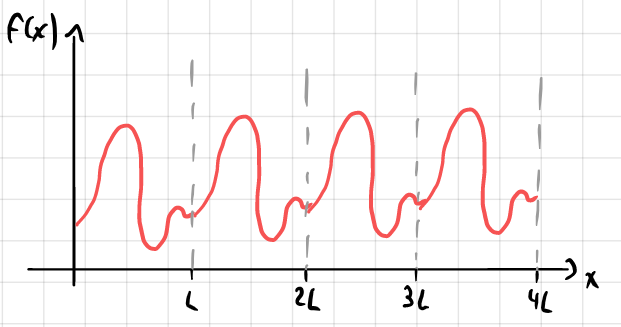
\includegraphics[width=0.7\linewidth]{Grafiken/2_Fourierreihen/Grafik1.PNG}
		\caption{Periodische Funktion mit Periodenlänge $L$}
		\label{}
	\end{figure}

	\begin{Def}
		Eine Funktion $f: \mathbb{R}\rightarrow\mathbb{R}(\mathbb{C})$ wird periodischen
		mit Periode $L$ , $L>0$, genannt wenn:
		$$f(x+L) = f(x) \quad \forall x \in \mathbb{R}$$
	\end{Def}

	\begin{Bem}
		Periodiesche Funktion mit Periode $L$ ist eindeutig auf ganz $\mathbb{R}$ fesgelegt,
		wenn man sie auf einem beliebiges Intervall der Länge $L$, $[a,a+L)$ kennt.\\
		Standardvorgabe:
		$$[0,L) \quad \textrm{oder} \quad [-\frac{L}{2}, \frac{L}{2})$$
	\end{Bem}

	\begin{Bem}
		$f(x)$ periodisch mit Periode $L$
		$$\Rightarrow \int_{-\frac{L}{2}}^{\frac{L}{2}} \,dx f(x) = \int_{a-\frac{L}{2}}^{a+\frac{L}{2}} \,dx f(x)$$
	\end{Bem}

	Betrachte Funktion $f: \mathbb{R}\rightarrow\mathbb{R}(\mathbb{C})$ mit
	\begin{enumerate}[label=(\roman*)]
		\item periodisch mit Periode L, d.h. $f(x+L) = f(x) \quad \forall x \in \mathbb{R}$
		\item Lebesque-integrierbar auf dem Periodizitätsintervall, dh $f \in L^1(-\frac{L}{2},\frac{L}{2})$ (schwächer als quadratintegrierbar)
	\end{enumerate}

	Betrachte Funktionen der Einfachheit halber für $L=2\pi$\\
	Die $\infty$-trigometrische Reihe
	$$FR(f)(x)= \frac{1}{2} a_0 + \sum_{n=1}^\infty (a_n \cos(n x) + b_n \sin(n x)) \quad \textrm{mit}$$
	$$a_n = \frac{1}{\pi} \int_{-\pi}^{\pi} \,dx f(x)\cos(nx) \quad n \geq 0 \quad n \in \mathbb{N}$$
	$$b_n = \frac{1}{\pi} \int_{-\pi}^{\pi} \,dx f(x)\sin(nx) \quad n>0 \quad n \in \mathbb{N}$$
	heißt Fourierreihe der Funktion $f$ mit den Fourierkoeffizienten $a_n$ und $b_n$.

	Konvergenz der Partialsummen

	$FR(f)(x)= \frac{1}{2} a_0 + \sum_{n=1}^N (a_n \cos(n x) + b_n \sin(n x))$

	muss beachtet werden.

	\begin{Bem}
		Wenn $f \in L^1(-\pi,\pi)$, dann stellt Fourierreihe eine Entwicklung nach der
		OGB

		$\{1, \sin(nx), \cos(nx); n \in \mathbb{N}\}$ auf $\sqrt{2}$ normiert $\Rightarrow \frac{1}{2}$ bei $a_0$

		bzgl. des Skalarprodukts

		$$\langle f,g \rangle =  \frac{1}{\pi} \int_{-\pi}^{\pi} \,dx \overline{f(x)} g(x)$$

		dar.

		$\Rightarrow FR(f)$ konvergiert in $L^2$-Norm (Konvergenz im Mittel)

		$$\lim_{n\rightarrow \infty} {\Vert f- FR_N(t) \Vert}_2 = 0$$
	\end{Bem}

	\begin{Satz}{Parsewal I}
		$$\Vert f \Vert^2 = \frac{1}{2} \vert a_0 \vert^2 + \sum_{n=1}^{\infty} \left(\vert a_n \vert^2 + \vert b_n \vert^2\right)$$
	\end{Satz}

	\subsubsection{Rechenregeln und Beispiele}
	\begin{enumerate}[label=(\roman*)]
		\item Allgemeines Periodizitätsintervall $(a,b)$
			$$FR(f)(x)= \frac{1}{2} a_0 + \sum_{n=1}^\infty \left( a_n \cos\left(\frac{2\pi n x}{b-a}\right) + b_n \sin\left(\frac{2\pi n x}{b-a}\right) \right)$$
			$$a_n = \frac{2}{b-a} \int_{a}^{b} \,dx f(x) \cos \left(\frac{2\pi n x}{b-a}\right) \quad n \geq 0$$
			$$b_n = \frac{2}{b-a} \int_{a}^{b} \,dx f(x) \sin \left(\frac{2\pi n x}{b-a}\right) \quad n>0$$	

		\item Integrale über ein symetrisches Integrationsintervall 
			$\left(-\frac{L}{2}, \frac{L}{2} \right)$ um Null verschwinden
			für ungerade Integranden:
			\begin{itemize}
				\item $f(x) \quad \textrm{ungerade} \Leftrightarrow f(x) = -f(-x)$ 
					$$\frac{2}{L} \int_{-\frac{L}{2}}^{\frac{L}{2}} \,dx \underbrace{\underbrace{f(x)}_{ungerade} \underbrace{\cos\left(\frac{2\pi}{L} n x\right)}_{gerade}}_{ungerade} = 0 \quad \cos()\textrm{-Terme verschwinden}$$
				\item $f(x) \quad \textrm{gerade} \Leftrightarrow f(x) = f(-x)$
					$$\frac{2}{L} \int_{-\frac{L}{2}}^{\frac{L}{2}} \,dx \underbrace{\underbrace{f(x)}_{gerade} \underbrace{\sin\left(\frac{2\pi}{L} n x\right)}_{ungerade}}_{ungerade} = 0 \quad \sin()\textrm{-Terme verschwinden}$$
			\end{itemize}
		\item Integrale über ein Vielfaches der Periode von $\sin$- oder 			$\cos$-Funktion verschwinden
			$$\int_{a}^{a+k\frac{L}{n}} \sin\left(\frac{2\pi}{L} n x\right) \,dx =
			\int_{a}^{a+k\frac{L}{n}} \cos\left(\frac{2\pi}{L} n x\right) \,dx = 0
			\quad k\neq 0 \quad n \neq 0$$
			\begin{figure}[H]
				\centering
				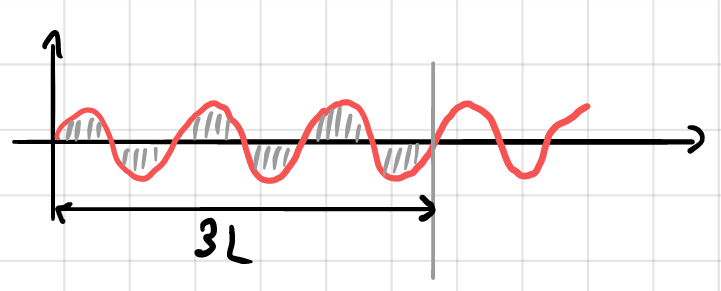
\includegraphics[width=0.4 \linewidth]{Grafiken/2_Fourierreihen/Grafik2.PNG}
			\end{figure}
		\item Linearität der Fourierreihe
			$$FR(f+g)(x) = FR(f)(x) + FR(g)(x)$$
			$$FR(\alpha \cdot f)(x) = \alpha \cdot FR(f)(x)$$
	\end{enumerate}
	
	\begin{Bsp}{Sägezahnfunktion}
		$$f(x)=x \quad x \in (-\pi,\pi) \quad \textrm{Periode: } 2\pi$$
		\begin{figure}[H]
			\centering
			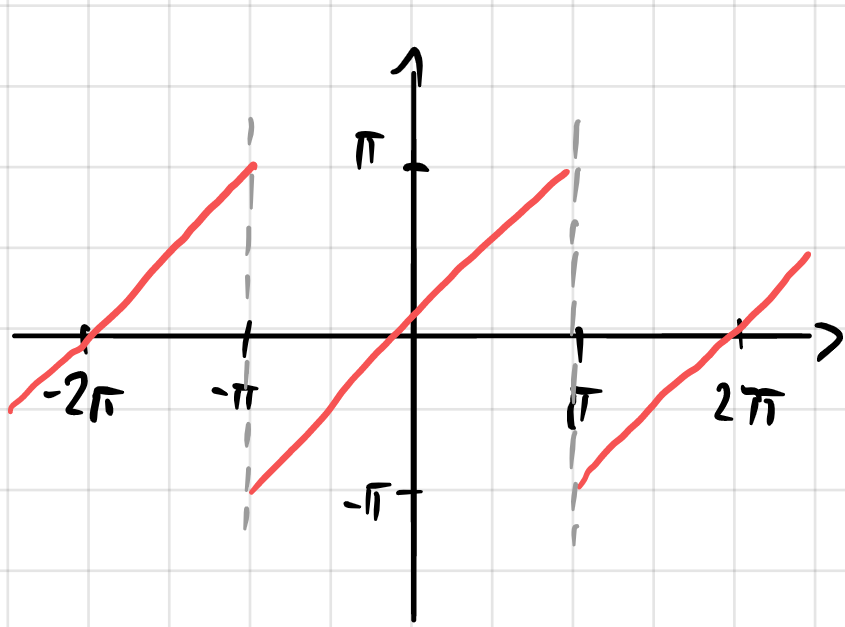
\includegraphics[width=0.4\linewidth]{Grafiken/2_Fourierreihen/Grafik3.PNG}
		\end{figure}

		$$a_{n \geq 0} = \frac{1}{\pi} \int_{-\pi}^{\pi} \,dx x \cos(nx) = 0$$

	\end{Bsp}

	%------3-INTEGRALTRANSFORMATION------%
	\section{Integral Transformationen}
    $f \in L^1[-\frac{L}{2}, \frac{L}{2}]$ lässt sich durch
    FR darstellen. Was passiert mit FR, wenn 
    $L \rightarrow \infty$ ?


    %ToDo
    \subsection{Testfunktionenräume und Distributionen}

    \begin{Def}
        V VR über $\mathbb{K}$. Ein Funktional $F$ ist eine Abbildung:
        $$F: V \rightarrow \mathbb{K}$$
        $$ \phi \in V \mapsto F(\phi) = \alpha \in \mathbb{K}$$

        Ein lineares Funktional $F$ erfüllt die Linearitätsbedingung
        $$F(\alpha \phi + \beta \psi) = \alpha F(\phi) + \beta F(\psi) \quad \phi , \psi \in V \quad \alpha, \beta \in \mathbb{K} $$

        Die Menge aller linerarer Funktionale auf $V$
        $$V^\ast =  \{ F | F:V \rightarrow \mathbb{K} \quad linear \} $$

        bildet selbst bzgl. der "punktweisen" Addition und Multiplikation
        mit einem Skalar einen VR, den algebraischen Dualraum von $V$.
        $$(F+G)(\phi) = F(\phi) + G(\phi) \quad \forall \phi \in V $$
        $$(\alpha F)(\phi) = \alpha (F)(\phi)  \quad \forall \alpha \in \mathbb{K} \quad \forall \phi \in V $$
    \end{Def}

    \begin{Def}
        Der Raum der beliebig oft stetig diff-baren (komplex- oder 
        reellwertigen) Funktionen mit kompakten Trägern ist definiert als
        $$C_0^\infty (\mathbb{R}^n)  := \{ f:\mathbb{R}^n \rightarrow \mathbb{C}(\mathbb{R}) | f \in C^\infty(\mathbb{R}^n) \textrm{ und } f(\vec{x})=0 \textrm{ für } \vec{x} \in \mathbb{R}^n \setminus  \Omega \textrm{ mit } \Omega \textrm{ kompakt} \}$$
        $$( \Omega \subset \mathbb{R}^n \textrm{ kompakt } \Rightarrow \Omega \textrm{ abgeschlossen und beschränkt} )$$

        Bsp: $\phi = \left\{ \begin{array}{ll}
            e^{\frac{1}{x^2-1}} & |x| < 1 \\
            0 & \, |x| \geq 1 \\
            \end{array}
            \right. \quad \in C_0^{\infty} $
    \end{Def}

    \begin{Def}{Konvergenz in $C_0^{\infty}(\mathbb{R}^n)$}
        Eine Funktionenfolge $(f_k)_{k \in \mathbb{N}} \subset C_0^{\infty}(\mathbb{R}^n)$ konvergiert gegen
        $f \in C_0^{\infty}(\mathbb{R}^n)$

    \end{Def}


	\newpage

	\listoftables
	\listoffigures
\end{document}
 